\documentclass[a4paper, 12pt]{article}
\usepackage[total={17cm,25cm}, top=2.5cm, left=2.5cm, right=2.5cm,  includefoot]{geometry}
\usepackage[utf8]{inputenc}
\usepackage{array}
\usepackage{multirow}
\usepackage{hhline}
\usepackage{gensymb}
\usepackage{graphicx}
\graphicspath{ {} }
\usepackage[czech]{babel}
\usepackage{enumitem}
\usepackage{pdfpages}
\usepackage{amsmath}
\usepackage{verbatim}
\usepackage{listings}
\usepackage{hyperref}
\usepackage{amssymb}


\pagestyle{empty} % vypne číslování stránek




%\usepackage[OT2,OT1]{fontenc}
\newcommand\cyr
{
\renewcommand\rmdefault{wncyr}
\renewcommand\sfdefault{wncyss}
\renewcommand\encodingdefault{OT2}
\normalfont
\selectfont
}
\DeclareTextFontCommand{\textcyr}{\cyr}
\def\cprime{\char"7E }
\def\cdprime{\char"7F }
\def\eoborotnoye{\char’013}
\def\Eoborotnoye{\char’003}


\begin{document}



\begin{titlepage}
\begin{center}
\noindent
\Large \textbf{České vysoké učení technické v Praze }\\ Fakulta stavební
\vspace{5cm}

\huge

%vložení loga cvut
%\begin{figure}[h!]
%	\centering
%	\includegraphics[width=7cm]{logo.png}
%\end{figure}

\vspace{0.5cm}

155ADKG: Množinové operace s polygony \\

\vspace{10cm}




\Large
Michael Kala\\
Anna Zemánková \\

\end{center}

\end{titlepage}




\pagestyle{plain}     % zapne obyčejné číslování
\setcounter{page}{1}  % nastaví čítač stránek znovu od jedné

%\tableofcontents
%\newpage

\section{Zadání}

\begin{figure}[h!]
	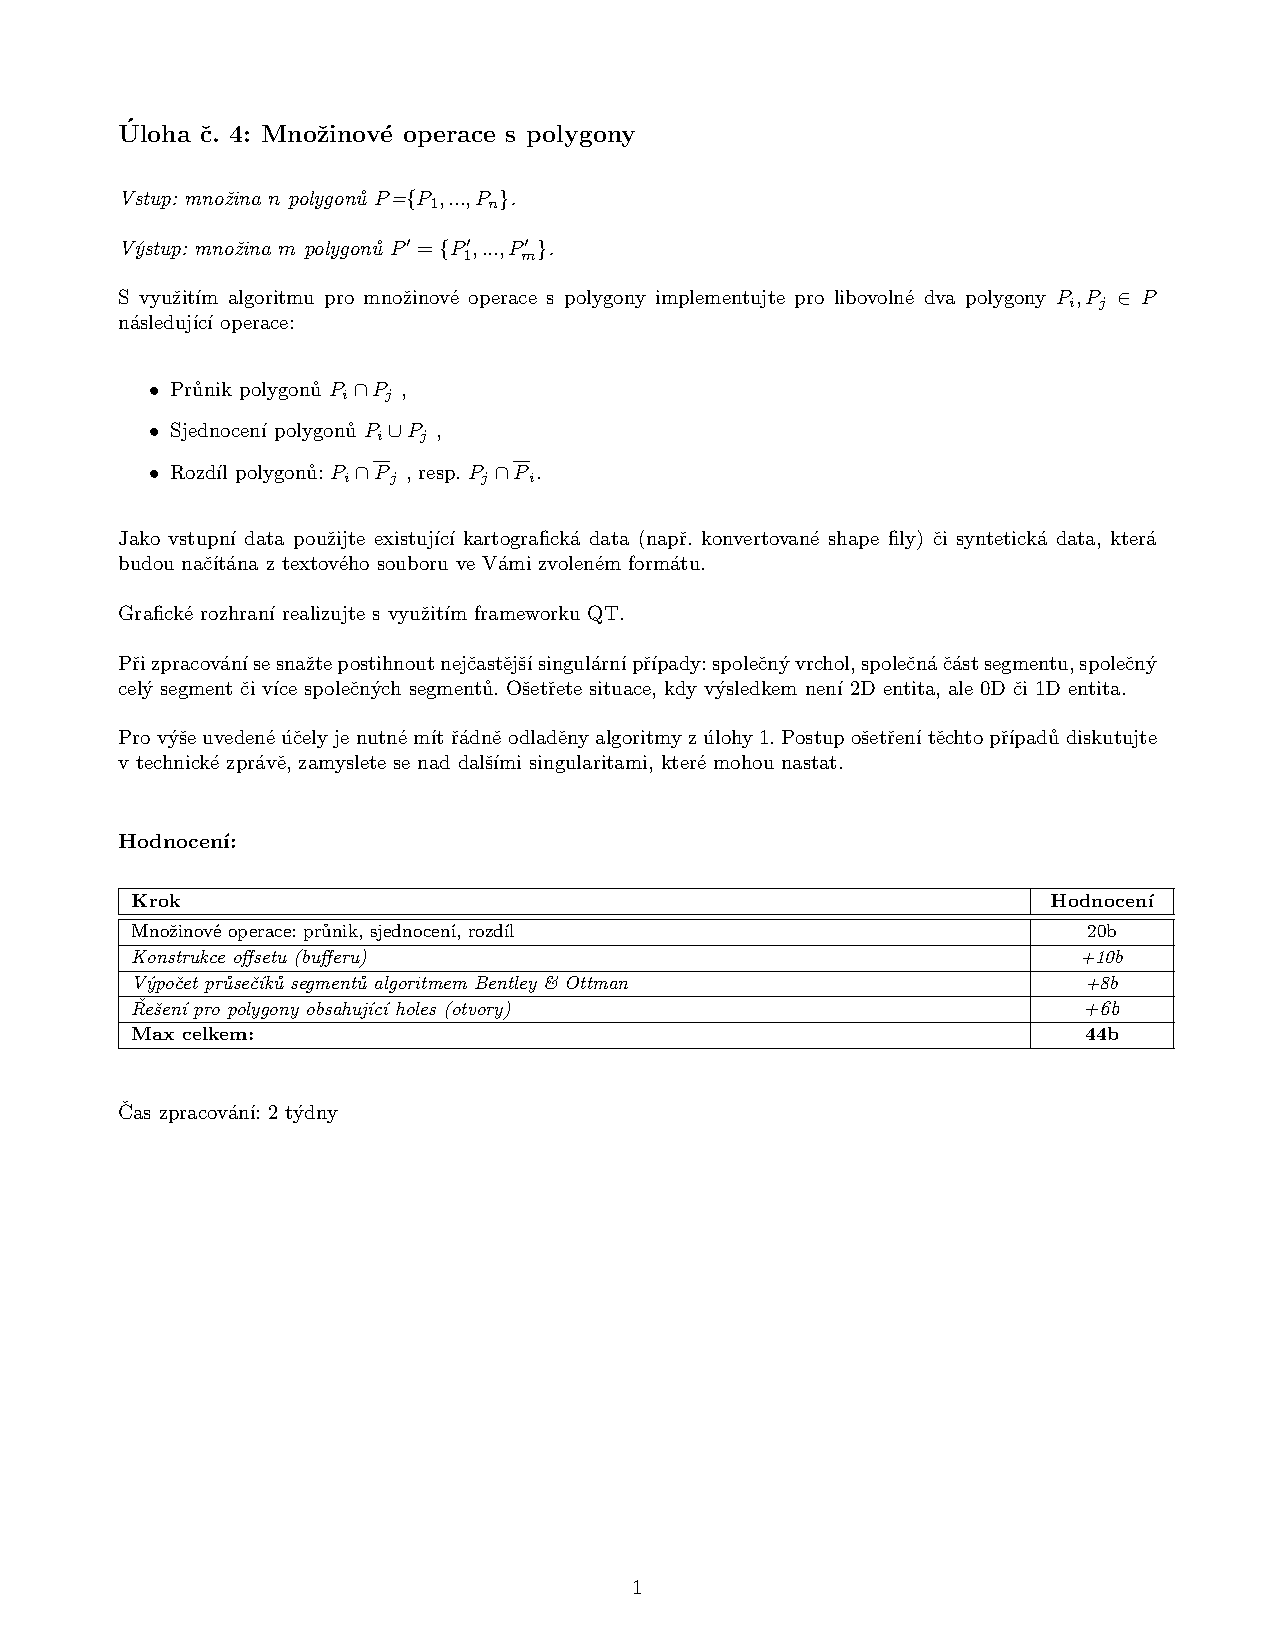
\includegraphics[clip, trim=0cm 4cm 0cm 3cm, width=1.0\textwidth]{zadani.pdf}
\end{figure}


\section{Údaje o bonusových úlohách}

V rámci této úlohy nebyly zpracovány žádné bonusy.



\clearpage

\section{Popis a rozbor problému}
Mějme dva polygony A $\{p_i\}$ a B $\{p_j\}$.\\

Množinové operace:
\begin{itemize}
\item Sjednocení (Union): $C = A \cup B$
\item Průnik (Intersection): $C = A \cap B$
\item Rozdíl (Difference): $C = A \cap \bar{B}$ nebo $C = B \cap \bar{A}$
\end{itemize}

%OBRÁZEK
\begin{figure}[h]
	\centering
	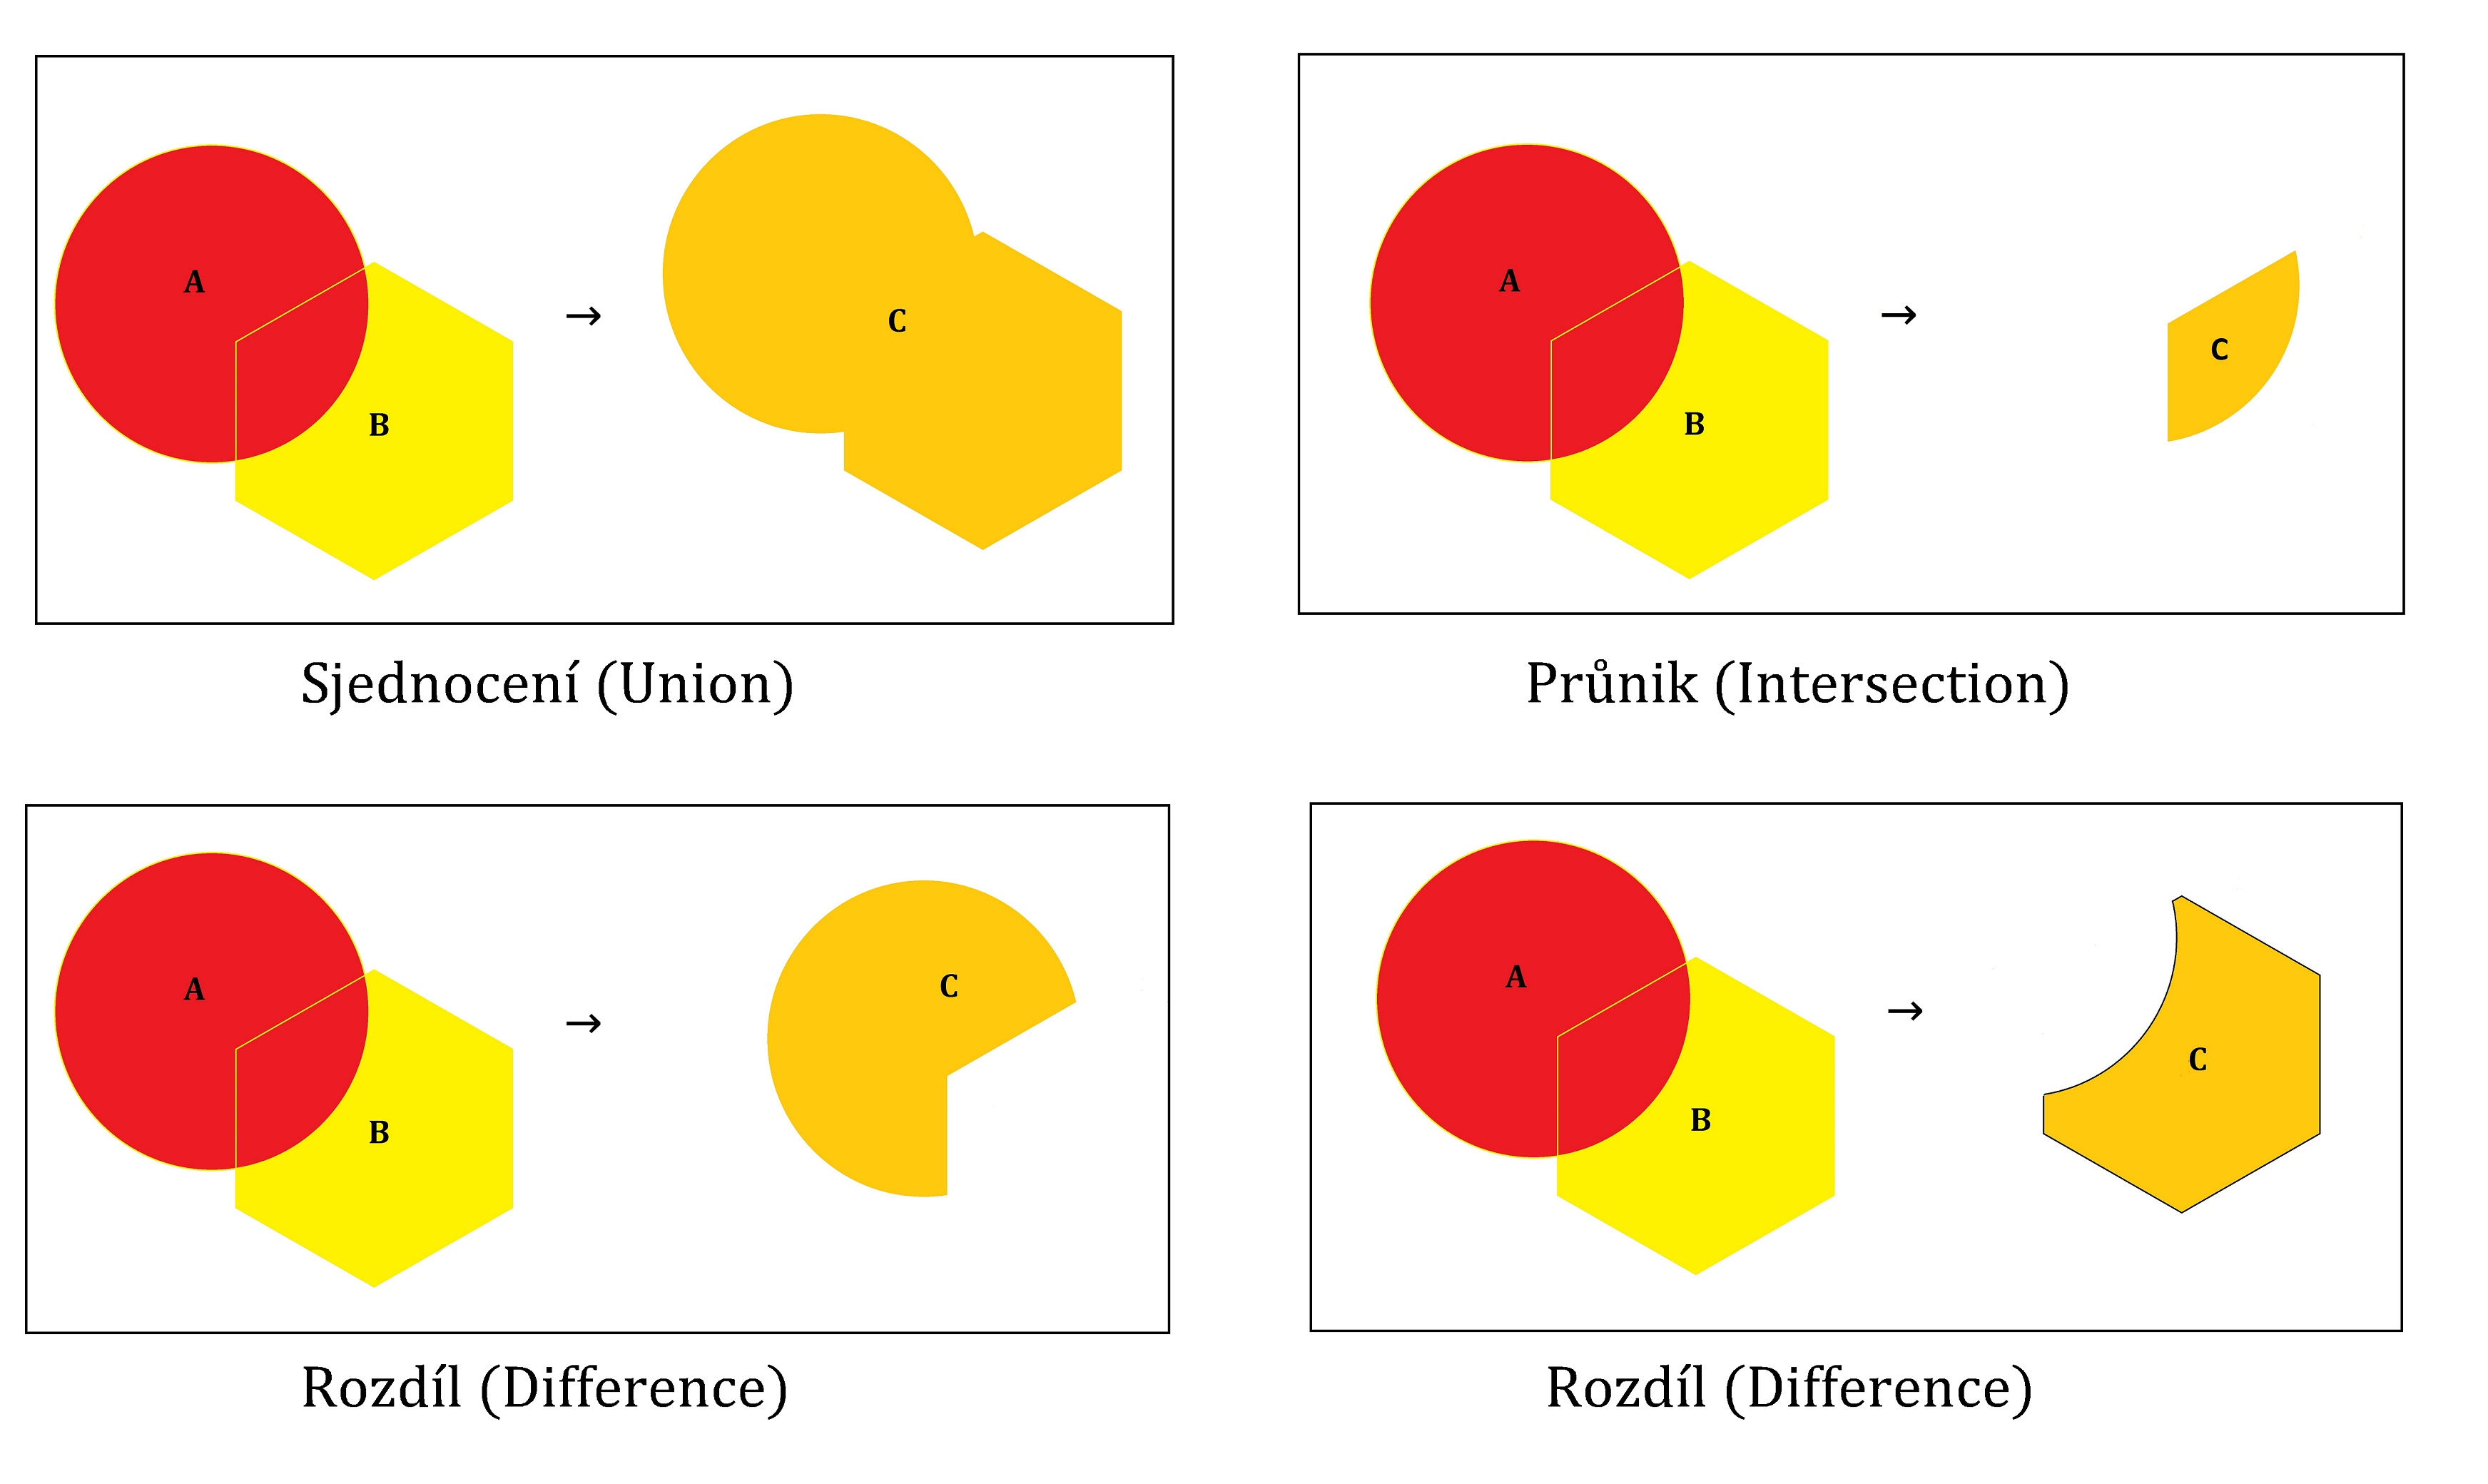
\includegraphics[width=18cm]{BO.jpg}
	\caption{Příklady množinových operací}
\end{figure}


\clearpage
\section{Popis algoritmů}

\subsection{Výpočet průsečíků}
Nejprve bylo třeba určit průsečíky množin A a B a setřídit je. Následně byly ohodnoceny vrcholy množiny A resp. B podle pozice vůči B resp. A. Poté byly dle ohodnocení vybrány vrcholy a z nich vytvořeny fragmenty. Nakonec byl(y) z fragmentů vytvořen(y) výsledný/é polygon(y).

\subsubsection{Implementace metody}
\begin{enumerate}
\item $ for (i = 0; i < n, i++) $ 
\item \hspace {1cm} $ M = map (double, QPointFB) $ // Vytvoření mapy 
\item \hspace {1cm} $ for (j = 0; j < m, j++) $
\item \hspace {2cm} if $ b_{ij} = (p_i, p_{(i+)1\%n} \cap q_j, q_{(j+)1\%m }) \neq 0$ // Existuje průsečík
\item \hspace {3cm} $ M [\alpha_i] \longleftarrow b_{ij}$ //Přidej do M
\item \hspace {3cm} ProcessIntersection $ (b_{ij}, \beta, B, j) $ //Zpracuj první průsečík pro $ e_j $
\item \hspace {1cm} if $(||M|| > 0)$ // Nějaké průsečíky jsme nalezli
\item \hspace{2cm} $  for \forall m \in M: $ // Procházej všechny průsečíky v M
\item  \hspace{3cm} $ b \longleftarrow m.second $ // Získej 2. hodnotu z páru
\item \hspace{3cm} ProcessIntersection $ (b, \alpha, A, i) $ //Zpracuj první průsečík pro $ e_i $
\end{enumerate}

\vspace{1cm}

\textbf{Process Intersection} 
\begin{enumerate}
	\item $ if (|t| < \epsilon): $ 
	\item \hspace {1cm} $ P[i] \longleftarrow inters $  //Startovní bod průsečíkem
	\item  $ if (|t-1| < \epsilon): $
	\item \hspace {1cm}  $ P[(i+1)\%m] \longleftarrow inters$ // Koncový bod průsečíkem
	\item  $ else:$
	\item \hspace {1cm} ProcessIntersection $ i \longleftarrow i+1 $ //Inkrementuj pozici
	\item \hspace {1cm} if $P \longleftarrow  (b,i)$ // Přidej průsečík na pozici i+1
\end{enumerate}

\clearpage

\subsection{Fragmenty}

\subsubsection{Vytvoření fragmentů - implementace metody}
\begin{enumerate}
	\item $ i \longleftarrow 0 $
	\item $ while (g(P[i]) \neq g \vee P[i] \neq inters) $ //Dokud P[i] není průsečík s orientací g
	\item \hspace{1cm} $ i \longleftarrow i+1 $
	\item $ if (i\equiv n) $ return; //Žádný bod s touto orientací neexistuje
	\item $ i_s \longleftarrow i $ //Zapamatuj startovní index prvního průsečíku
	\item $ do $
	\item \hspace{1cm} $ f = \emptyset $ //Prázdný fragment
	\item \hspace{1cm} $ if (createFragmentFromVertices (i_s, P, g, i f)) $ //Nalezen fragment
	\item \hspace{2cm} $ if (s) f.reverse() $ //Swapuj prvky fragmentu, je-li třeba
	\item \hspace{2cm} $ F[f[0]] \longrightarrow f $ //Přidej fragment do mapy, klíč poč. bod
	\item \hspace{1cm} $ i \longleftarrow (i+1)\%m $
	\item $ while (i \neq i_s) $ //Dokud nedojdeme k počátečnímu průsečíku
\end{enumerate}

\vspace{1cm}

\textbf{createFragmentFromVertices}

\begin{enumerate}
	\item  $ if (g(P[i]) \neq g \vee P[i] \neq inters) $ //Bod není průsečíkem s orientací g
	\item \hspace{1cm} $ return $ $ false $ 
	\item for (;;) 
	\item \hspace{1cm} $  f \longleftarrow P[i] $ // Přidej bod do fragmentu
	\item \hspace{1cm} $ i \longleftarrow (i+1)\%n $
	\item \hspace{1cm} $ if (i \equiv i_s) $ //Obešli jsme celý polygon
	\item \hspace{2cm} $ return$  $ false $ 
	\item \hspace{1cm} $ if (g(P[i]) \neq g)  $ // První bod s rozdílou orientací
	\item \hspace{2cm} $ f \longleftarrow P[i] $ //Přidej ho do seznamu
	\item \hspace{2cm} $ return$  $true $

\end{enumerate}

\clearpage

\subsubsection{Sestavení oblastí z fragmentů - implementace metody}
\begin{enumerate}
	\item $ for \forall f \in F $
	\item \hspace{1cm} $ P \longleftarrow \emptyset $ //Vytvoř prázdný polygon
	\item \hspace{1cm} $ s \longleftarrow f.first $ //Najdi startovní bod fragmentu
	\item \hspace{1cm} $ if (!f.second.first) $ //Pokud fragment již nebyl zpracován
		\item \hspace{2cm} $ if (createPolygonFROMFragments(s,F,P)) $ 
			\item \hspace{3cm} $ C \longleftarrow P $ //Přidej polygon do seznamu	
\end{enumerate}

\vspace{1.5cm}
\subsubsection{Vytvoření polygonu z fragmentů  - implementace metody}

\begin{enumerate}
	\item  $ QPoint n \longleftarrow s $ //Inicializuj následující bod
	\item for (;;) //Projdi všechyn fragmenty tvořící polygon
	\item \hspace{1cm} $ f \longleftarrow F.find(n) $ //Najdi navazující fragment
	\item \hspace{1cm} $ if (f \equiv F.end) $ // Fragment s takovým poč. bodem neexistuje
	\item \hspace{2cm} $ return$ $ false $
	\item \hspace{1cm} $ f.second.first \longleftarrow true $ //Fragment označen za zpracovaný
	\item \hspace{1cm} $ n \longleftarrow f.second.second.back() $ // Najdi následující bod
	\item \hspace{1cm} $ P \longleftarrow f.second.second - \{f.second.second[0]\}() $ // Přidej bez poč. bodu
	\item \hspace{1cm} $ if (n \equiv s) $ // Obešli jsme polygon, jsme na startu
	\item \hspace{2cm} $ return$  $true $
\end{enumerate}

\clearpage

\subsection{Množinové operace}

\subsubsection{Implementace metody}
\begin{enumerate}
	\item if $ (o(A) != CCW) $
	\item \hspace{1cm} $ A.switchOr() $ // Změň orientaci na CCW
	\item if $ (o(B) != CCW) $
	\item \hspace{1cm} $ B.switchOr() $ // Změň orientaci na CCW
	\item $ ComputeIntersections(A,B) $ // urči průsečíky A,B
	\item $ SetPositions (A,B) $ //Urči polohu vrcholů vůči oblastem
	\item $map <QPointFB, pair <bool, vector<QPointFB>>> F$
	\item $ pos1 = (oper \equiv intersection \vee oper \equiv DifAB?Inner:Outer) $
	\item $ pos2 = (oper \equiv intersection \vee oper \equiv DifAB?Inner:Outer) $
	\item $ swap1 = (oper \equiv DifAB? : true : false) $
	\item $ swap2 = (oper \equiv DifAB? : true : false) $
	\item $ CreateFragments (A, pos1, swap1, F) $
	\item $ CreateFragments (B, pos2, swap2, F) $
	\item $ MergeFragments (A,B,C) $
\end{enumerate}

\clearpage
% ===============================================================

\section{Problematické situace}

Problematické jsou polygony obsahující otvory - bylo by třeba speciální ošetření pro tyto případy. Jinak by mohlo dojít k tomu, že například při opraci Union bude do výsledku zahrnuta celá oblast včetně otvorů jakoby tam nebyly.
\clearpage

\section{Vstupní data}

Dva polygony mohou být "nakresleny" klikáním do kanvasu pokud je zakšrnutá možnost \textit{Draw polygons}, pomocí tlačítka \textit{Polygon A/B} lze přepínat mezi polygony.\\

\noindent Dále mohou být polygony nahrány pomocí tlačítka \textit{Load polygon}, v tom případě jsou data nahrána ze vstupního souboru *.txt, kde jsou souřadnice lomových bodů polygonů v tomto pořadí:
\begin{enumerate}
\item	počet bodů v prvním polygonu 
\item	 souřadnice X a Y (s desetinnou tečkou, pokud se nejedná o celé číslo) bodů prvního polygonu
\item	 počet bodů v druhém polygonu
\item souřadnice X a Y bodů druhého polygonu atd.
\end{enumerate}

Př.: Vstupní soubor se 2 polygony, kde první polygon obsahuje 6 bodů a druhý polygon 5 bodů bude vypadat následovně:\\
 
\noindent 6 5 10 20 5 20 40 30 12 39 46 15 48\\
5 2 25 25 20 50 30 23 51 22 43\\

Vše může být zapsáno do jednoho řádku, odděleno mezerami nebo jako v příkladu výše může každý útvar začínat na novém řádku.\\

%\vspace{1cm}
\section{Výstupní data}
Výsledek aplikace je zobrazen graficky na kanvasu (červenou barvou).

\begin{figure}[h]
	\centering
	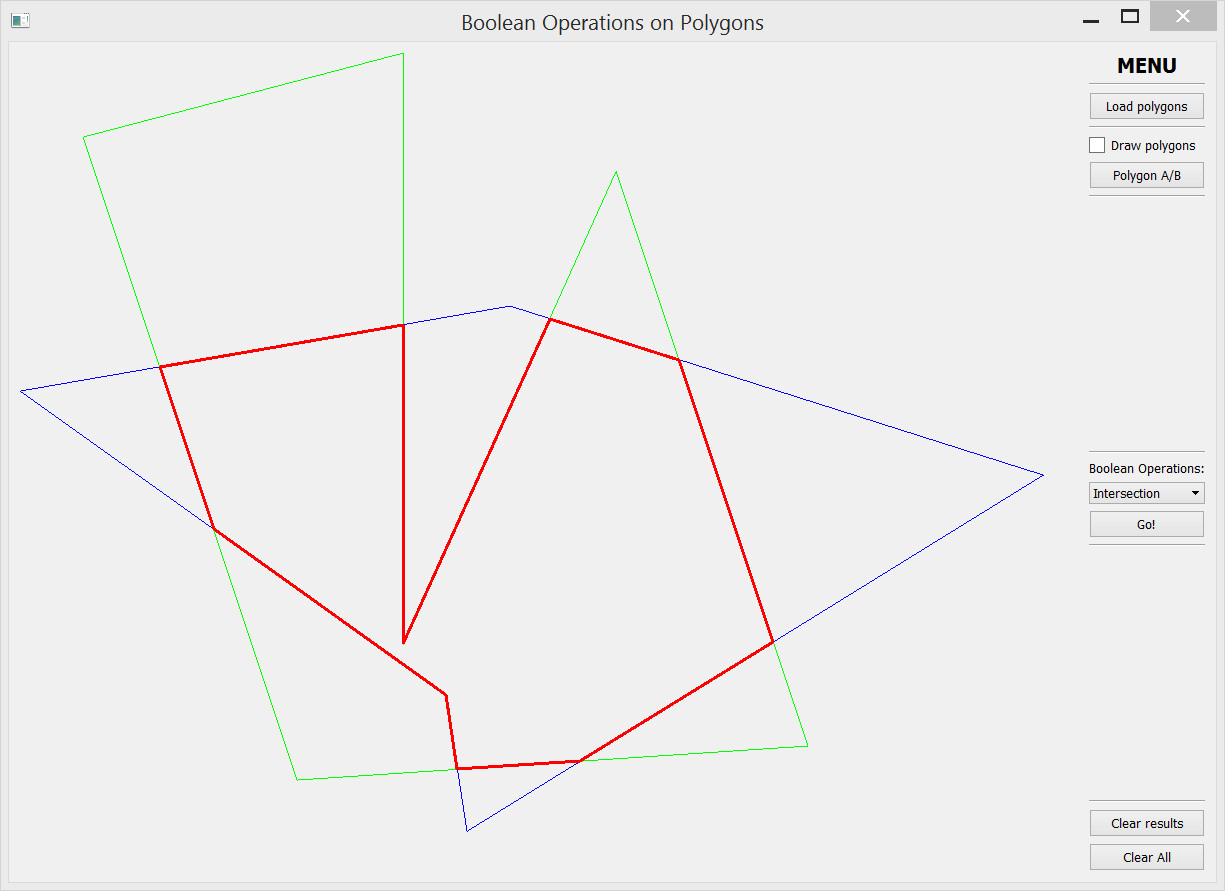
\includegraphics[width=10cm]{inter.jpg}
	\caption{Intersection}
\end{figure}
\clearpage
%--------------------------------------------------------------------------------------------------------------------------------------
\section{Ukázka vytvořené aplikace}
\begin{figure}[h]
	\centering
	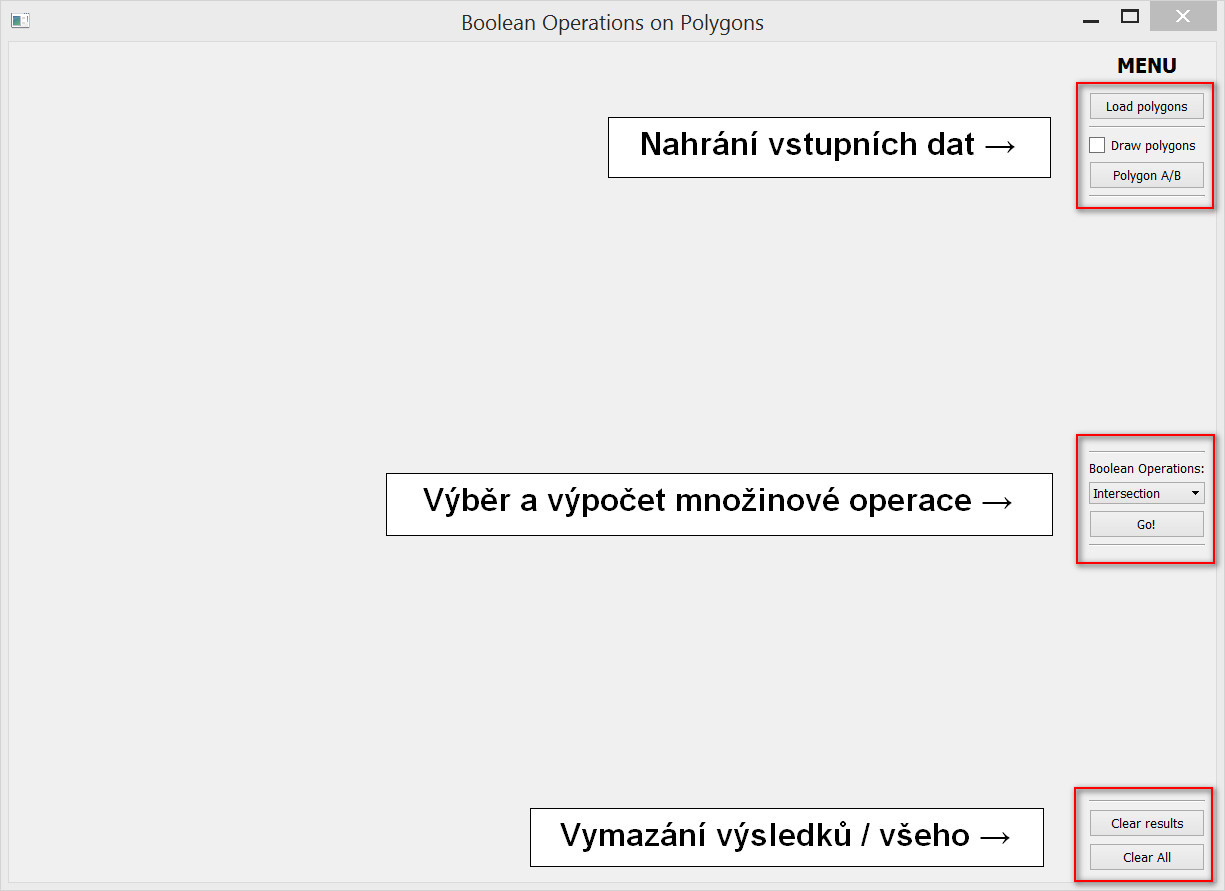
\includegraphics[width=10cm]{ap.jpg}
	\caption{Aplikace}
\end{figure}

%OBRÁZEK
\begin{figure}[h]
	\centering
	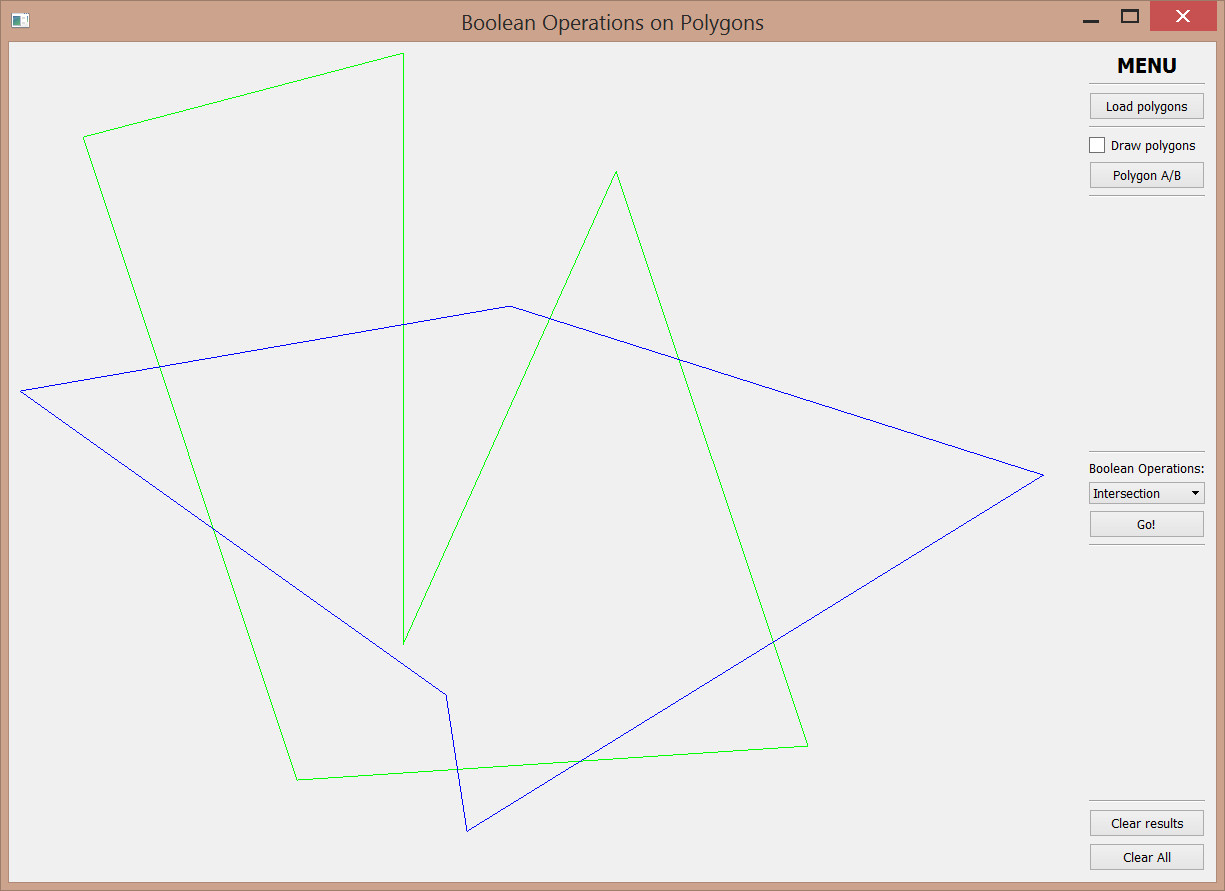
\includegraphics[width=10cm]{vstup.jpg}
	\caption{Nahrání vstupních dat}
\end{figure}

\begin{figure}[h]
	\centering
	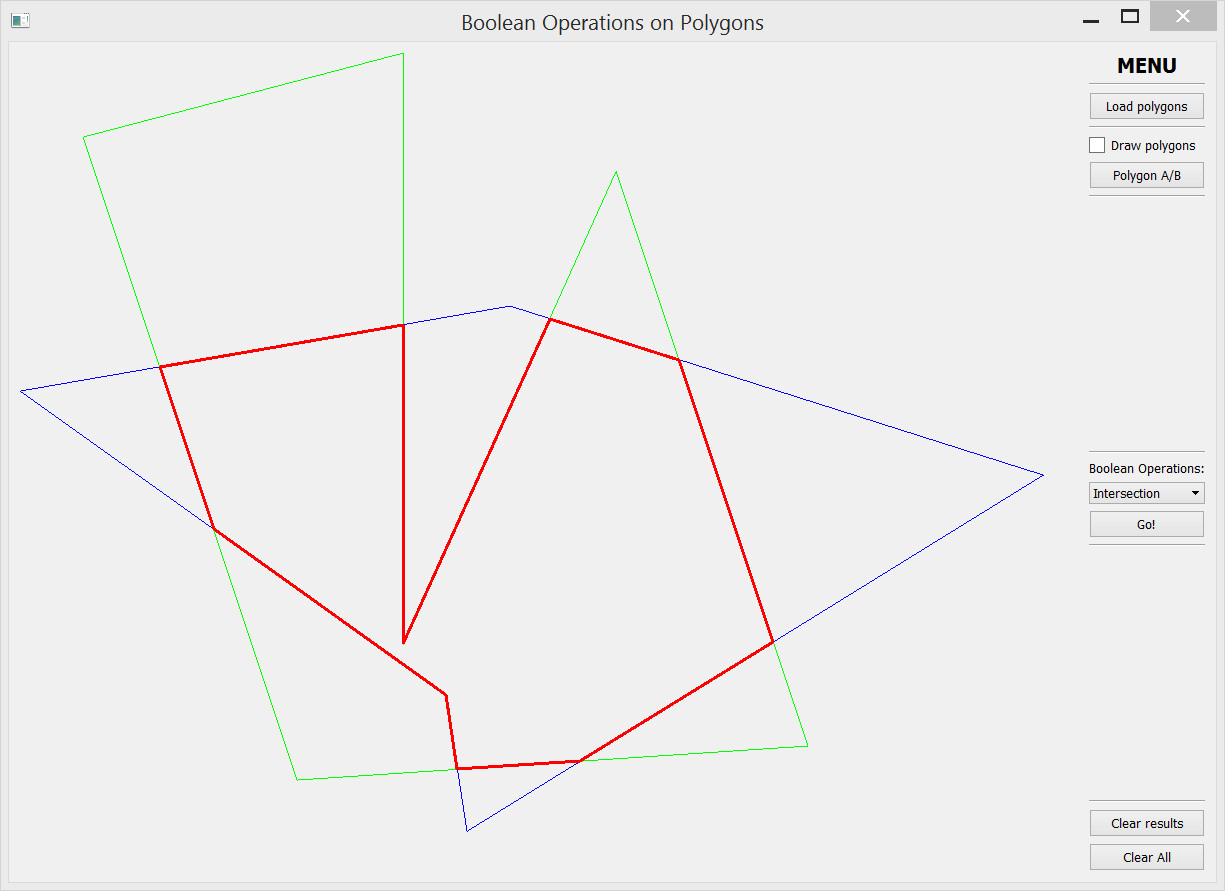
\includegraphics[width=12cm]{inter.jpg}
	\caption{Intersection}
\end{figure}

\begin{figure}[h]
	\centering
	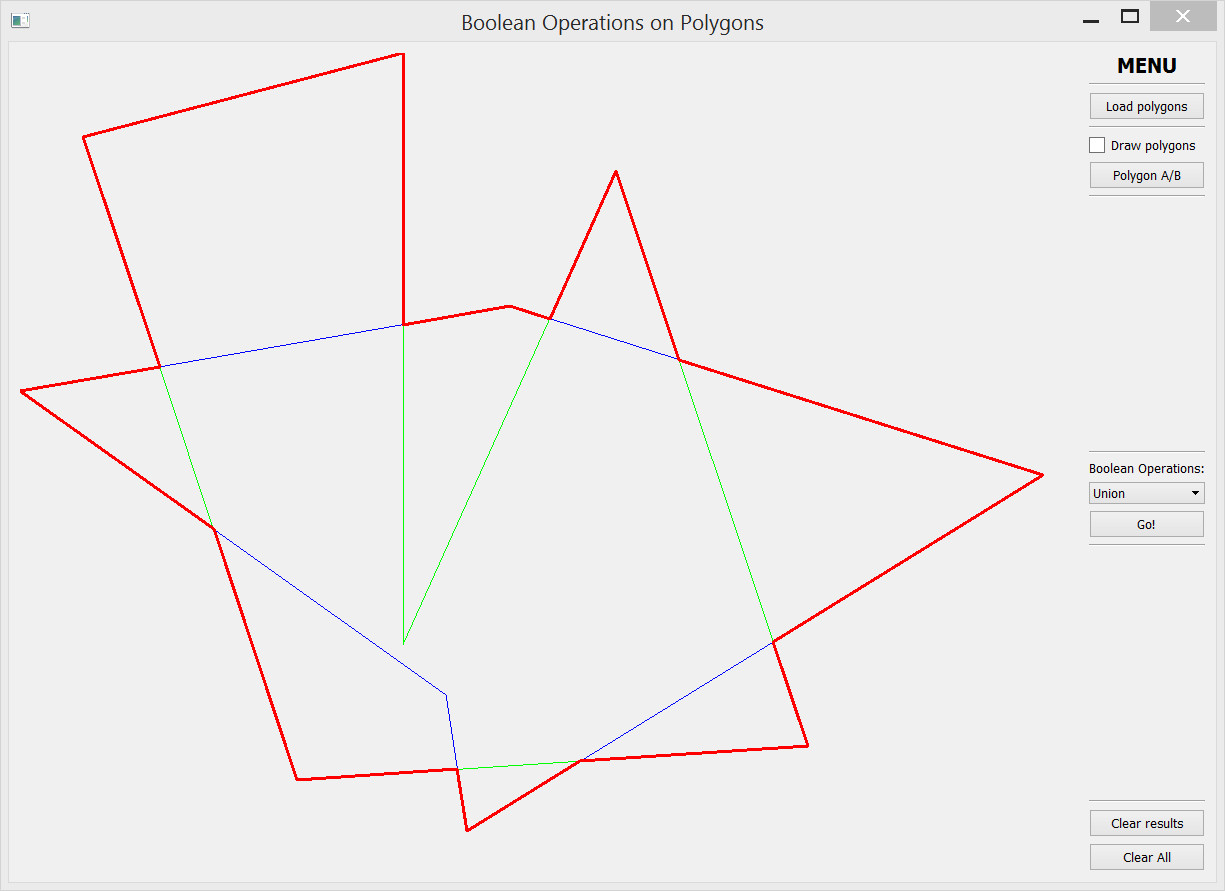
\includegraphics[width=12cm]{union.jpg}
	\caption{Union}
\end{figure}

\begin{figure}[h]
	\centering
	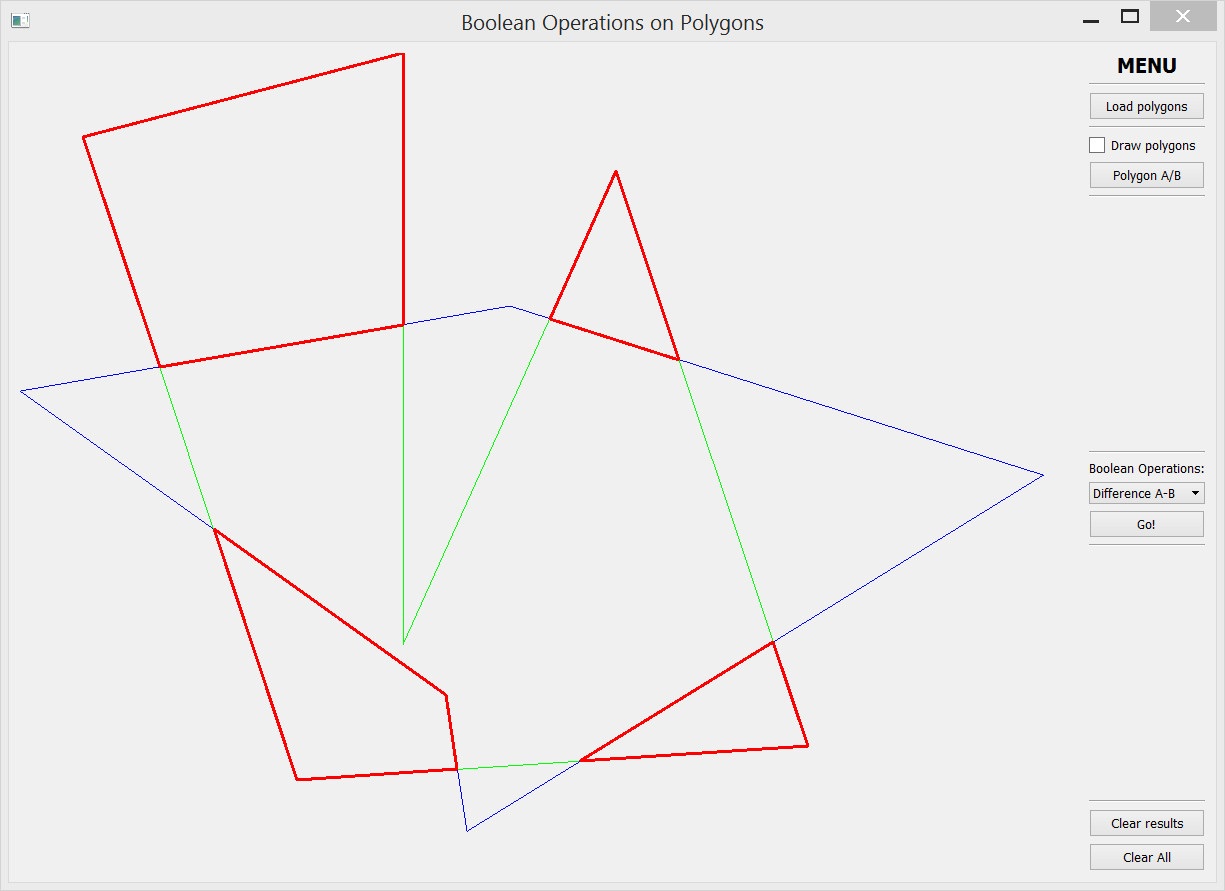
\includegraphics[width=12cm]{A-B.jpg}
	\caption{Difference A-B}
\end{figure}


\begin{figure}[h]
	\centering
	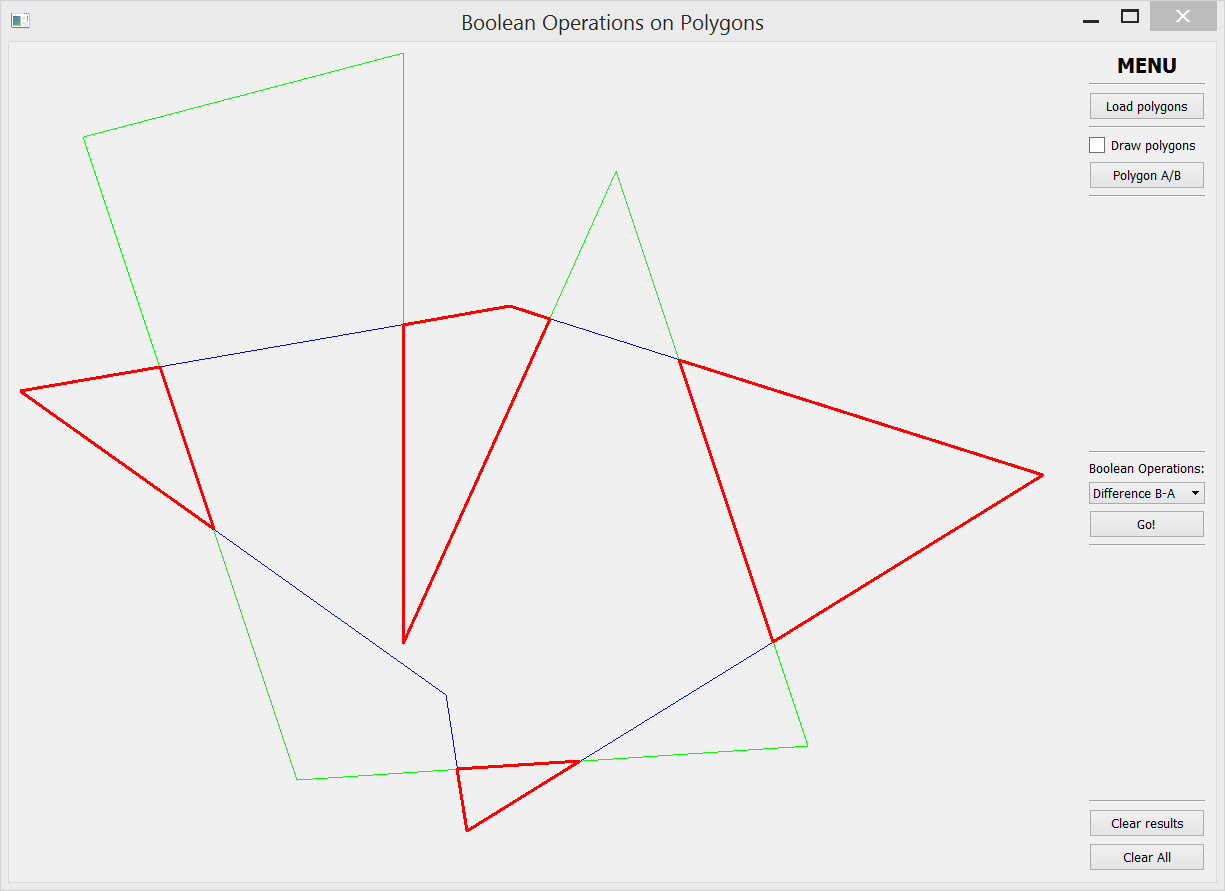
\includegraphics[width=12cm]{B-A.jpg}
	\caption{Difference B-A}
\end{figure}


\clearpage

%=======================================================================================


\section{Dokumentace}

\subsection{Types}
Tato třída je využita k definici výčtových typů použitých jako návratové hodnoty v algoritmech použitých v aplikaci.
\begin{itemize}
	\item Výčtový typ \textbf{TPointPolygon}.
	\begin{itemize}
		\item \textit{INSIDE, OUTSIDE, ON}
	\end{itemize}
	\item Výčtový typ \textbf{TBooleanOperation}.
	\begin{itemize}
		\item \textit{INTERSECTION, UNION, DIFFAB, DIFFBA}
	\end{itemize}
	\item Výčtový typ \textbf{T2LinesPosition}.
	\begin{itemize}
		\item \textit{PARALLEL, COLINEAR, INTERSECTIONG, NONINTERSECTING}
	\end{itemize}
	\item Výčtový typ \textbf{TPointLinePosition}.
	\begin{itemize}
		\item \textit{LEFT, RIGHT, COL}
	\end{itemize}
\end{itemize}

\subsection{QPointFB}
Definice nového datového typu \textbf{QPointFB}, který dědí od třídy \textbf{QPointF}.
\begin{itemize}
	\item	Členské proměnné \textbf{alfa, beta} - parametry popisující polohu bodu vůči dvěma přímkám (implicitně nastavené na 0), jejich typem je \textbf{double}
	\item Členská proměnná \textbf{inters} - \textbf{bool}ovská proměnná indikující, zda jde o průsečík, implicitně nastavené na \textit{false}
	\item Členská proměnná \textbf{pos} - indikuje polohu bodu vůči polygonu, jejím typem je \textbf{TPointPolygon}, impicitně nastavené na \textit{ON}
	\item Public metody - getery
	\begin{itemize}
		\item \textbf{getAlfa, getBeta, getInters, getPosition} - získání členských proměnných
	\end{itemize}
	\item Public metody - setery
	\begin{itemize}
		\item \textbf{setAlfa, setBeta, setInters, setPosition} - nastavení hodnot členských proměnných
	\end{itemize}
\end{itemize}

\subsection{Algorithms}
V této třídě jsou staticky implementovány metody pro výpočet množinových operací. 

\begin{itemize}
	\item Metoda \textbf{getPositionWinding}
		\begin{itemize}
			\item Tato metoda slouží k určení polohy bodu vůči polygonu pomocí Winding algoritmu. Jejím návratovým typem je \textbf{TPointPolygon}. Vstupem je bod \textbf{QPointFB q} a polygon \textbf{std::vector$<$QPointFB$>$ pol}, jejichž vzájemná poloha je určována.
		\end{itemize}
	\item Metoda \textbf{getPointLinePosition}
		\begin{itemize}
			\item Tato metoda slouží k určení polohy bodu vůči linii. Jejím návratovým typem je \textbf{TPointLinePosition}. Vstupem jsou body \textbf{QPointFB q, a, b}.
		\end{itemize}
	\item Metoda \textbf{get2LinesAngle}
		\begin{itemize}
			\item Metoda sloužící k výpočtu úhlu mezi 2 liniemi. Jejím návratovým typem je \textbf{double}. Vstupem jsou body určující linie: \textbf{QPointFB p1, p2, p3, p4}.
		\end{itemize}
	\item Metoda \textbf{get2LinesPosition}
		\begin{itemize}
			\item Tato metoda slouží k určení vzájemné polohy dvou linií. Jejím návratovým typem je \textbf{T2LinesPosition}. Na vstupu jsou body \textbf{QPointFB p1, p2, p3, p4} a bod \textbf{QPointFB intersection} obsahující případně vypočtený průsečík (předává se referencí). 
		\end{itemize}
	\item Metoda \textbf{computePolygonIntersections}
		\begin{itemize}
			\item Metoda sloužící k výpočtu průsečíků dvou polygonů. Jejím návratovým typem je \textbf{void}. Na vstupu jsou 2 polygony \textbf{std::vector$<$QPointFB$>$ p1, p2}.
		\end{itemize}
	\item Metoda \textbf{processIntersection}
		\begin{itemize}
			\item Metoda pro processing vypočtených průsečíků z metody \textbf{computePolygonIntersections}. Slouží pro správné zařazení průsečíků do seznamu. Jejím návratovým typem je \textbf{void}. Na vstupu je vypočtený průsečík \textbf{QPointFB b}, hodnota jeho parametru \textbf{alfa/beta}, oblast zpracování \textbf{std::vector$<$QPointFB$>$ poly} a index počátečního bodu hrany \textbf{int i}.
		\end{itemize}
	\item Metoda \textbf{setPositions}
		\begin{itemize}
			\item Metoda sloužící k určení polohy středních bodů jednotlivých hran vstupních polygonů vzhledem k druhému z polygonů. Návratovým typem je \textbf{void}. Na vstupu jsou oba vstupní polygony \textbf{std::vector$<$QPointFB$>$ pol1, pol2}.
		\end{itemize}
	\item Metoda \textbf{createFragments}
		\begin{itemize}
			\item Metoda sloužící k vytvoření fragmentů ze sousedních bodů o stejném ohodnocení. Fragmenty ukládá do mapy. Jejím návratovým typem je \textbf{void}. Na vstupu je 	polygon bodů \textbf{std::vector$<$QPointFB$>$ pol}, \textbf{TPointPolygon pol} - ohodnocení bodů, \textbf{bool swap} - orientace fragmentu, \textbf{std::map $<$QPointFB, std::pair$<$bool,  std::vector$<$QPointFB$> >$ $>$ fragments} - mapa fragmentů.
		\end{itemize}
	\item Metoda \textbf{createFragmentsFromVertices}
		\begin{itemize}
			\item Pomocná metoda metody \textbf{createFragments} pro výpočet fragmentů. Výstupním typem je \textbf{bool} detekující, zda-li se fragment vypočetl. Na vstupu je index počátečního bodu fragmentu \textbf{int i\_start}, body polygonu \textbf{std::vector$<$QPointFB$>$ pol}, ohodnocení bodů \textbf{TPointPolygon pos}, index daného bodu \textbf{int i} a seznam bodů fragmentu (měněn referencí) \textbf{std::vector$<$QPointFB$>$ fr}.
		\end{itemize}
	\item Metoda \textbf{mergeFragments}
		\begin{itemize}
			\item Metoda sloužící ke spojení fragmentů do výsledného polygonu a uložení do seznamu polygonů. Návratovým typem je \textbf{void}. Na vstupu je mapa fragmentů \textbf{std::map$<$QPointFB, std::pair$<$bool, std::vector$<$QPointFB$> > >$ FR} a vektor vektorů bodů výsledných polygonů \textbf{std::vector$<$std::vector$<$QPointFB$> >$ res}
		\end{itemize}
	\item Metoda \textbf{createPolygonFromFragments}
		\begin{itemize}
			\item Metoda sloužící k vytvoření polygonu z fragmentů. Výstupním teypem je \textbf{bool} indikující, zda byl polygon vytvořen. Na vstupu je startovní bod fragmentu \textbf{QPointFB start}, mapa fragmentů \textbf{std::map$<$QPointFB, std::pair$<$bool, std::vector$<$QPointFB$> > >$ FR}, vektor bodů vytvářeného polygonu \\ \textbf{std::vector$<$QPointFB$>$ pol}.
		\end{itemize}			
	\item Metoda \textbf{getPolygonOrientation}
		\begin{itemize}
			\item Tato metoda slouží k výpočtu výměry polygonu pomocí LLH vzorce a tedy k určení orientace bodů polygonu. Typem výstupu je \textbf{double} určující výměru a znaménkem orientaci polygonu. Na vstupu je polygon \textbf{std::vector$<$QPointFB$>$ pol}.
		\end{itemize}			
	\item Metoda \textbf{BooleanOper}
		\begin{itemize}
			\item Zastřešující metoda pro výpočet množinových operacích. Na výstupu je vektor zjištěných polygonů typu \textbf{std::vector$<$std::vector$<$QPointFB$> >$}. Na vstupu jsou dva polygony, nad nimiž jsou operace počítány: \textbf{std::vector$<$QPointFB$>$ A, B} a zvolený typ operace \textbf{TBooleanOperation oper}. 
		\end{itemize}
	\item Metoda \textbf{resetIntersections}
		\begin{itemize}
			\item Metoda, která slouží pro zresetování atributu průsečíku u bodů polygonu (tj. nastavení na \textit{false}). Výstupním typem je \textbf{void}. Na vstupu je polygon \\ \textbf{std::vector$<$QPointFB$>$ A}. 
		\end{itemize}
\end{itemize}

\subsection{Draw}
Třída Draw slouží k vykreslení načtených polygonů a polygonů vypočtených množinovými operacemi. Třída dědí od třídy \textbf{QWidget}. 

\begin{itemize}
	\item Členské proměnné \textbf{std::vector$<$QPointFB$>$ polA, polB} - vstupní polygony
	\item Členská proměnná \textbf{std::vector$<$std::vector$<$QPointFB$> >$ res} - výsledné polygony.
	\item Členská proměnná \textbf{bool ab} - flag značící, který ze vstupních polygonů je právě "naklikáván".
	\item Členská proměnná \textbf{bool draw\_pol} - flag značící, zda-li je zvolena možnost vstupu bodů polygonů pomocí klikání do kanvasu.
	\item Metoda \textbf{paintEvent}
		\begin{itemize}
			\item Tato metoda slouží k vykreslení načtených (nebo naklikaných) polygonů a výsledných polygonů. Metoda se volá pomocí metody \textbf{repaint()}. Návratovým typem je \textbf{void}. Na vstupu je \textbf{QPaintEvent *e}.
		\end{itemize}
	\item Metoda \textbf{drawPol}
	\begin{itemize}
		\item Pomocná metoda pro vykreslení polygonu. Výstupním typem je \textbf{void}. Na vstupu je vykreslovaný polygon \textbf{std::vector$<$QPointFB$>$ pol} a objekt handlující vykreslování \textbf{QPainter painter}.
	\end{itemize}
	\item Metoda \textbf{mousePressEvent}
		\begin{itemize}
			\item Metoda zajišťující uložení naklikaných bodů do příslušných polygonů. Výstupním typem je \textbf{void}, na vstupu je \textbf{QMouseEvent *e}.
		\end{itemize}
	\item Metoda \textbf{setAB}
		\begin{itemize}
			\item Metoda, kterou je zaměňován polygon, do něhož se ukládají naklikané body.
		\end{itemize}
	\item Metody \textbf{clearAll} resp. \textbf{clearResults}
		\begin{itemize}
			\item Vyčištění proměnných obsahujících vstupní a výsledné polygony resp. výsledné polygony. Výstupními typy jsou \textbf{void}.
		\end{itemize}
	\item Členské metody - setery
		\begin{itemize}
			 \item Metody \textbf{setRes} resp. \textbf{setA} resp. \textbf{setB} sloužící pro uložení polygonů do příslušných členských proměnných \textbf{res} resp. \textbf{polA} resp. \textbf{polB}.
		\end{itemize}
	\item Členské metody - getery
		\begin{itemize}
			\item Metody \textbf{getA} resp. \textbf{getB} vracející dané polygony \textbf{polA} resp. \textbf{polB}.
		\end{itemize}
	\item Metoda \textbf{setDrawPol}
		\begin{itemize}
			\item Metoda sloužící ke změné flagu \textbf{draw\_pol}
		\end{itemize}
	\item Metoda \textbf{loadPoints}
		\begin{itemize}
			\item Metoda sloužící k načení polygonů ze souboru. Výstupním typem je \textbf{void}. Na vstupu je \textbf{std::string points\_path} - cesta k souboru a \textbf{QSizeF canvas\_size} - velikost kanvasu.
		\end{itemize}
\end{itemize}


\subsection{Widget}
Tato třída slouží ke komunikaci s GUI. Třída dědí od třídy QWidget. Všechny její metody slouží jako sloty k signálům z GUI, nemají žádné vstupní hodnoty a jejich návratovým typem je void. 

\begin{itemize}
	\item Metoda \textbf{on\_pushButton\_clicked}
		\begin{itemize}
			\item Změna polygonu, do něhož se ukládají naklikané body.
		\end{itemize}
	\item Metoda \textbf{on\_pushButton\_2\_clicked}
		\begin{itemize}
			\item Provedení zvolené množinové operace.
		\end{itemize}
	\item Metoda \textbf{on\_pushButton\_3\_clicked}
		\begin{itemize}
			\item Vyčištění kanvasu od výsledku množinových operací.
		\end{itemize}
	\item Metoda \textbf{on\_pushButton\_4\_clicked}
		\begin{itemize}
			\item Vyčištění kanvasu od vstupních a výsledných polygonů.
		\end{itemize}
	\item Metoda \textbf{on\_draw\_poly\_check\_clicked}
		\begin{itemize}
			\item Nastavení, zda-li jde body vkládat klikáním.
		\end{itemize}
	\item Metoda \textbf{on\_load\_button\_clicked}
		\begin{itemize}
			\item Otevření file dialogu, načtení souboru se vstupními polygony.
		\end{itemize}
\end{itemize} 

\clearpage

\section{Přílohy}

\begin{itemize}
	\item Příloha č.1: Vstupní data - \textit{body.txt}
\end{itemize}

\section{Závěr}
Tato úloha byla z celého semestru nejobtížnější a (i vzhledem k volnu přes Vánoce) hůře jsme se v kódu orientovali. Také proto jsme nebyli schopní přijít na to, jak vše odladit, i když jsme si nad tím lámali hlavu.


\subsection{Návrhy na vylepšení}
Jako první se nabízí nedokončený offset, dále pak bonusová úloha pro polygony s otvory a již zvýšené odladění - např. ošetření situací, kdy je výsledkem bod či úsečka.


\clearpage
\section{Zdroje}

\begin{enumerate}
\item  BAYER, Tomáš. Konvexní obálky [online][cit. 3.1.2019]. \\
Dostupné z: https://web.natur.cuni.cz/~bayertom/images/courses/Adk/adk9.pdf  \\

\item  BAYER, Tomáš. Konvexní obálky [online][cit. 3.1.2019]. \\
Dostupné z: https://web.natur.cuni.cz/~bayertom/images/courses/Adk/adkcv4.pdf\\
%=======================================================================================
\end{enumerate}
\end{document}



 
